\section{Acoustic Bump}

% Describe test case
% - open-closed tube, with a central DNS region and upstream and downstream acoustic regions modelled by ADCBC, like figure ..
% - Fluid defined by: T_0 = 298 K, p_0 = 1 bar, W = 28 kg / kmol, Pr = 0.7, c_p = 1100 J / kg / K, u_in = 0.2 m / s
% - A J_1 bump in the middle (easy to calculate approximately under linearity assumption) which travels to the left in the DNS region to begin with
% - Enforce ADCBC inflows and outflows in a thin DNS region to approximate the 1D acoustic problem as with a 2D domain
% - The full reacting Navier-Stokes equations are solved in the DNS region as a precursor to a flame being in the DNS region. The boundary conditions also work almost identically in this case under the viscous, inert, isothermal equations which are also implemented in the SUNSET code, but are not used here.
% - For thin regions like this the averaging along the boundary makes sense, but as the DNS domain widens, it seems reasonable that this averaging would result in more and more inaccuracy (and difficulty due to instability...), so the similar method where queues are used for each boundary node should instead be used in wider domains. For all the cases in this report, the averaging procedure is used and we find good results regardless.


% Acoustic bump results
% - Show result of a Gaussian bump leaving the domain and reentering after 1 bounce, 2 bounce (each boundary) and 100 bounces for different sample periods and interpolation orders?
% Technically we should be modelling the acoustics using the convected wave equation, not the wave equation for quiescent fluids, however the Mach number is so low in this case O(10^-3) that the resulting effects are asymptotically unimportant.


% Different interpolation orders:
% - Constant interpolation maintains the quality of acoustic bump surprisingly well, whilst the non-constant interpolation seems to introduce some small error on every reentry of the acoustic bump
% - assuming it isn't the fault of a mistake in the sunset implementation, it seems like it shouldn't be caused by the boundary averaging procedure given that the fields are initialised and remain virtually one-dimensional the whole time. It is likely the rest of the method then regardless of averaging which contains some error which cancel out when constant values are used but doesn't for non-constant values?






\section{Acoustic Standing Wave}

% Describe test case
% - An acoustic standing wave. DNS region calculated by initialising the pressure field to a sinusoid, and the upstream/downstream regions are initialised by specifying values of L within the queue initially. Usually these queues would have been initialised as empty -- instead they are given corresponding L_1/5 values
% - other than this the code is ran in the same way

% Instability issue!
% - We observed that under certain boundary discretisations, a wringing instability of u develops at the inflow after many acoustic periods. This grows exponentially, suggesting the instability behaves linearly, until the vorticity produced within the DNS region destroys the solution
% - Show image!!
% - This instability can be reduced by increasing the coefficient of the hyperviscosity filter at the inflow boundary nodes. Specifically, by increasing the hyperviscosity tangential to the inflow, the wringing mode is dampened to the point that it cannot grow
% - for us, we..
% - This instability may or may not show up when multiple queues are used for each inflow/outflow, so this needs to be investigated. It appears to be largely a result of the boundary averaging procedure.

% Sampling error
% - We can also see the sampling instability in the standing wave results as a q-wave \cite{poinsot2001TheoreticalNumericalCombustion} which is largest at maximum values of L???
% - Show image/s. Easiest to see when instability is not present
% - We can find similar results for standing waves as a bump in terms of interpolation order?
% - Once again, for tubes which are long enough this should not be a concern due to the quadratic growth of period with length. This is consistent with our results in the next section

% Moving domain results
% - shows validation that the delay time can indeed change
% - time scale for delay change is much longer due to the low Mach number
% - in theory, the time delay can change faster, provided it doesn't exceed the sound speed (so multiple L values are not entering the domain at any one sample time)
% - Show two images at separate times where the domain has moved but the acoustic remains well-resolved




\section{Thermoacoustically Unstable Flame}

% UPDATE IMAGE TO:
% - use constant resolution
\begin{figure}[t]
\centering
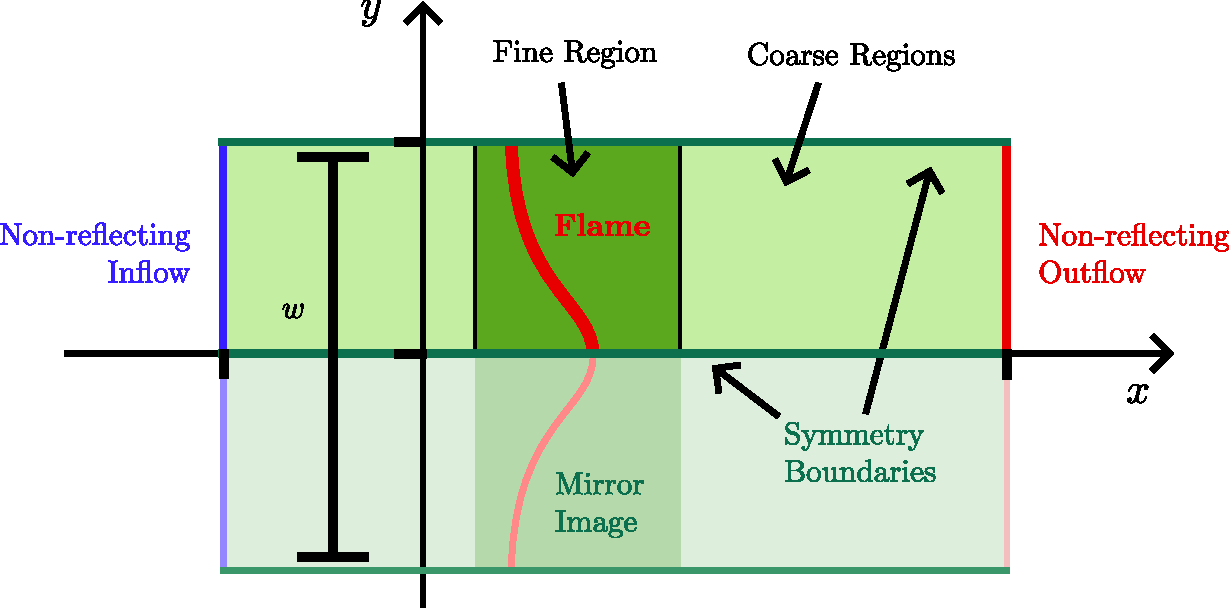
\includegraphics[scale=0.65]{assets/imgs/DNS-computational-domain.pdf}
\caption{DNS COMPUTATIONAL DOMAIN}
\label{fig:DNS-domain}
\end{figure}

\begin{figure}[t]
\centering
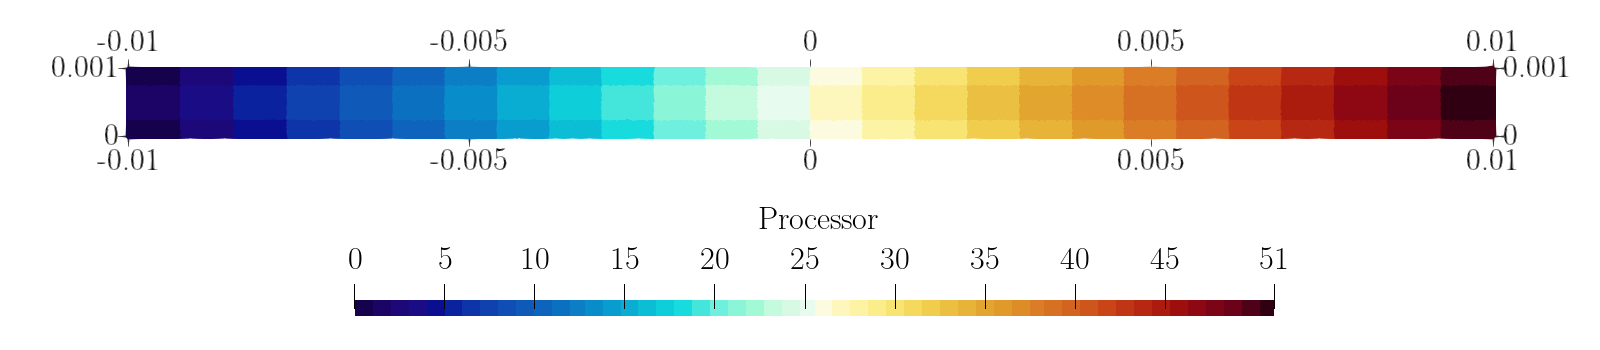
\includegraphics[scale=0.3]{assets/graphs/flame-sim-discretisation.png}
\caption{DNS COMPUTATIONAL DOMAIN}
\label{fig:disc1}
\end{figure}

\begin{figure}[t]
\centering
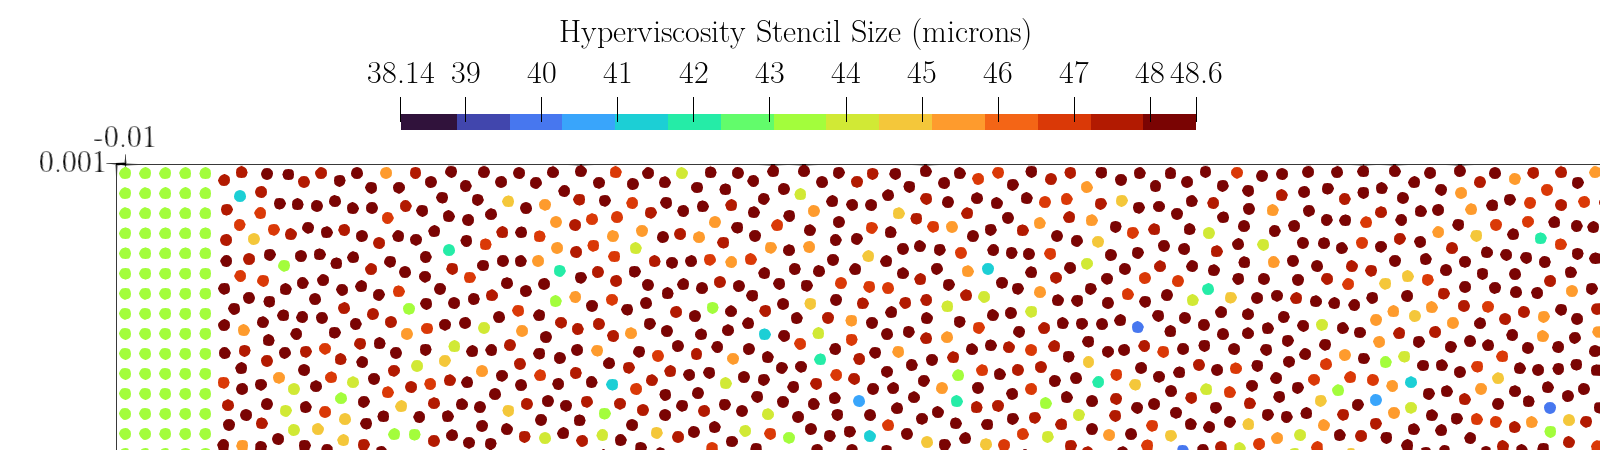
\includegraphics[scale=0.3]{assets/graphs/flame-sim-discretisation_zoom.png}
\caption{DNS COMPUTATIONAL DOMAIN}
\label{fig:disc2}
\end{figure}

% We now study a thermoacoustically unstable flame in a reflected DNS domain shown in fig ..
% Flame properties are: single step irreversible reaction with fluid properties constant in reactants and products, q = 6, Ze = 5, S_L = u_in = 0.2 m / s, Le = 1, with derived laminar flame thickness l_th = 0.216 mm
% Even though LABFM enables variable resolutions, we use constant discretisation length scale for these simulations as we don't know where the flame will end up a priori. A discretisation length scale of $s = 18$ μm is used and w = 2mm.
% Show the discretisation used zoomed in and out!
% It may seem like a large jump to go from inert, essentially isothermal acoustics to fully reacting flame-acoustic interactions, but the sunset code is designed with flame simulations in mind, so the simulations are 'easy' to perform having already implemented ADCBC.
% (Maybe there are better intermediate test cases? D-TDIBC don't seem to need them)



% Prediction from Eigenmodes
% - First we predict what results we get in a one-dimensional closed-open tube of the same length under the linear acoustic approximation, modelling the flame as a discontinuity which does not interact with the acoustics.
% First take the non-dimensionalised equations for compressible, inviscid fully non-linear flow:
% ... (continue on with maths)

\begin{figure}[t]
\centering
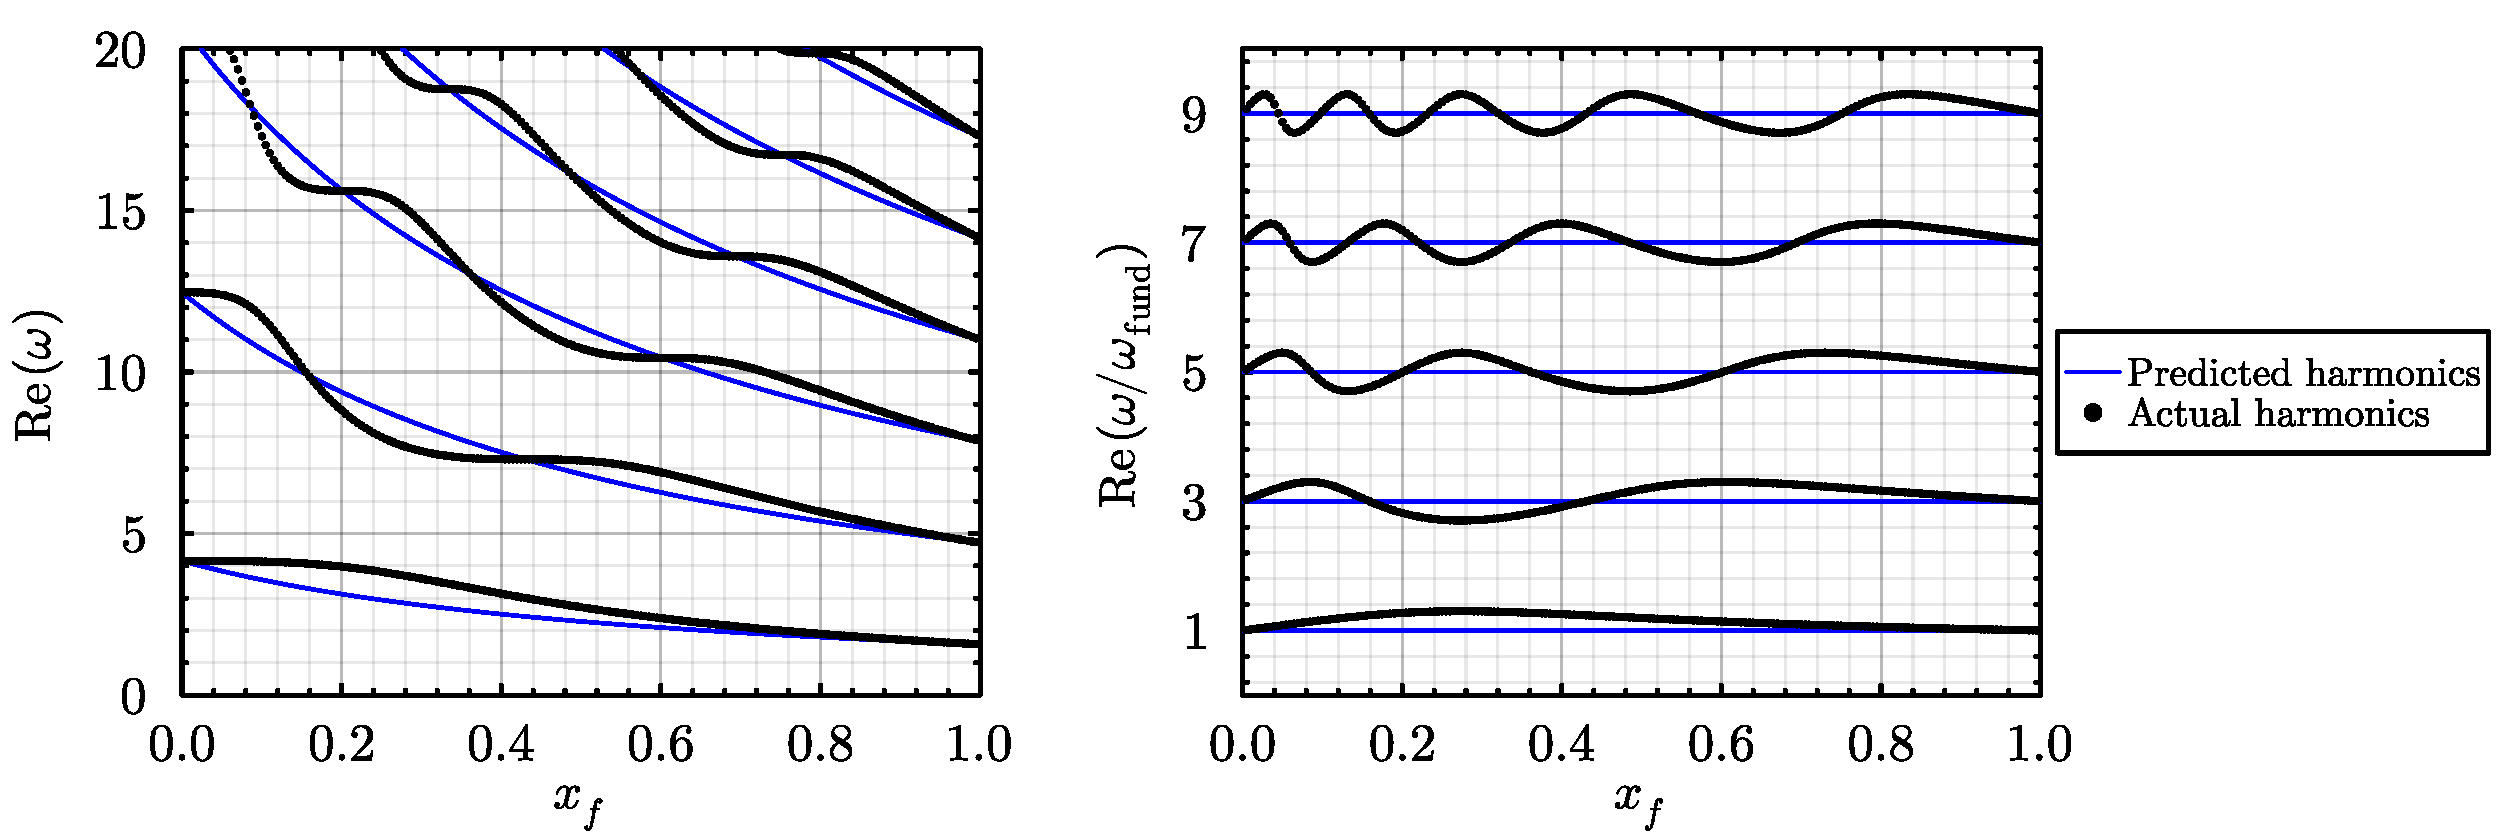
\includegraphics[scale=0.35]{assets/graphs/r=7_harmonics_both.pdf}
\caption{$r = 7$, LEFT: , RIGHT: divided by }
\label{fig:flame-harmonics}
\end{figure}

\begin{figure}[t]
\centering
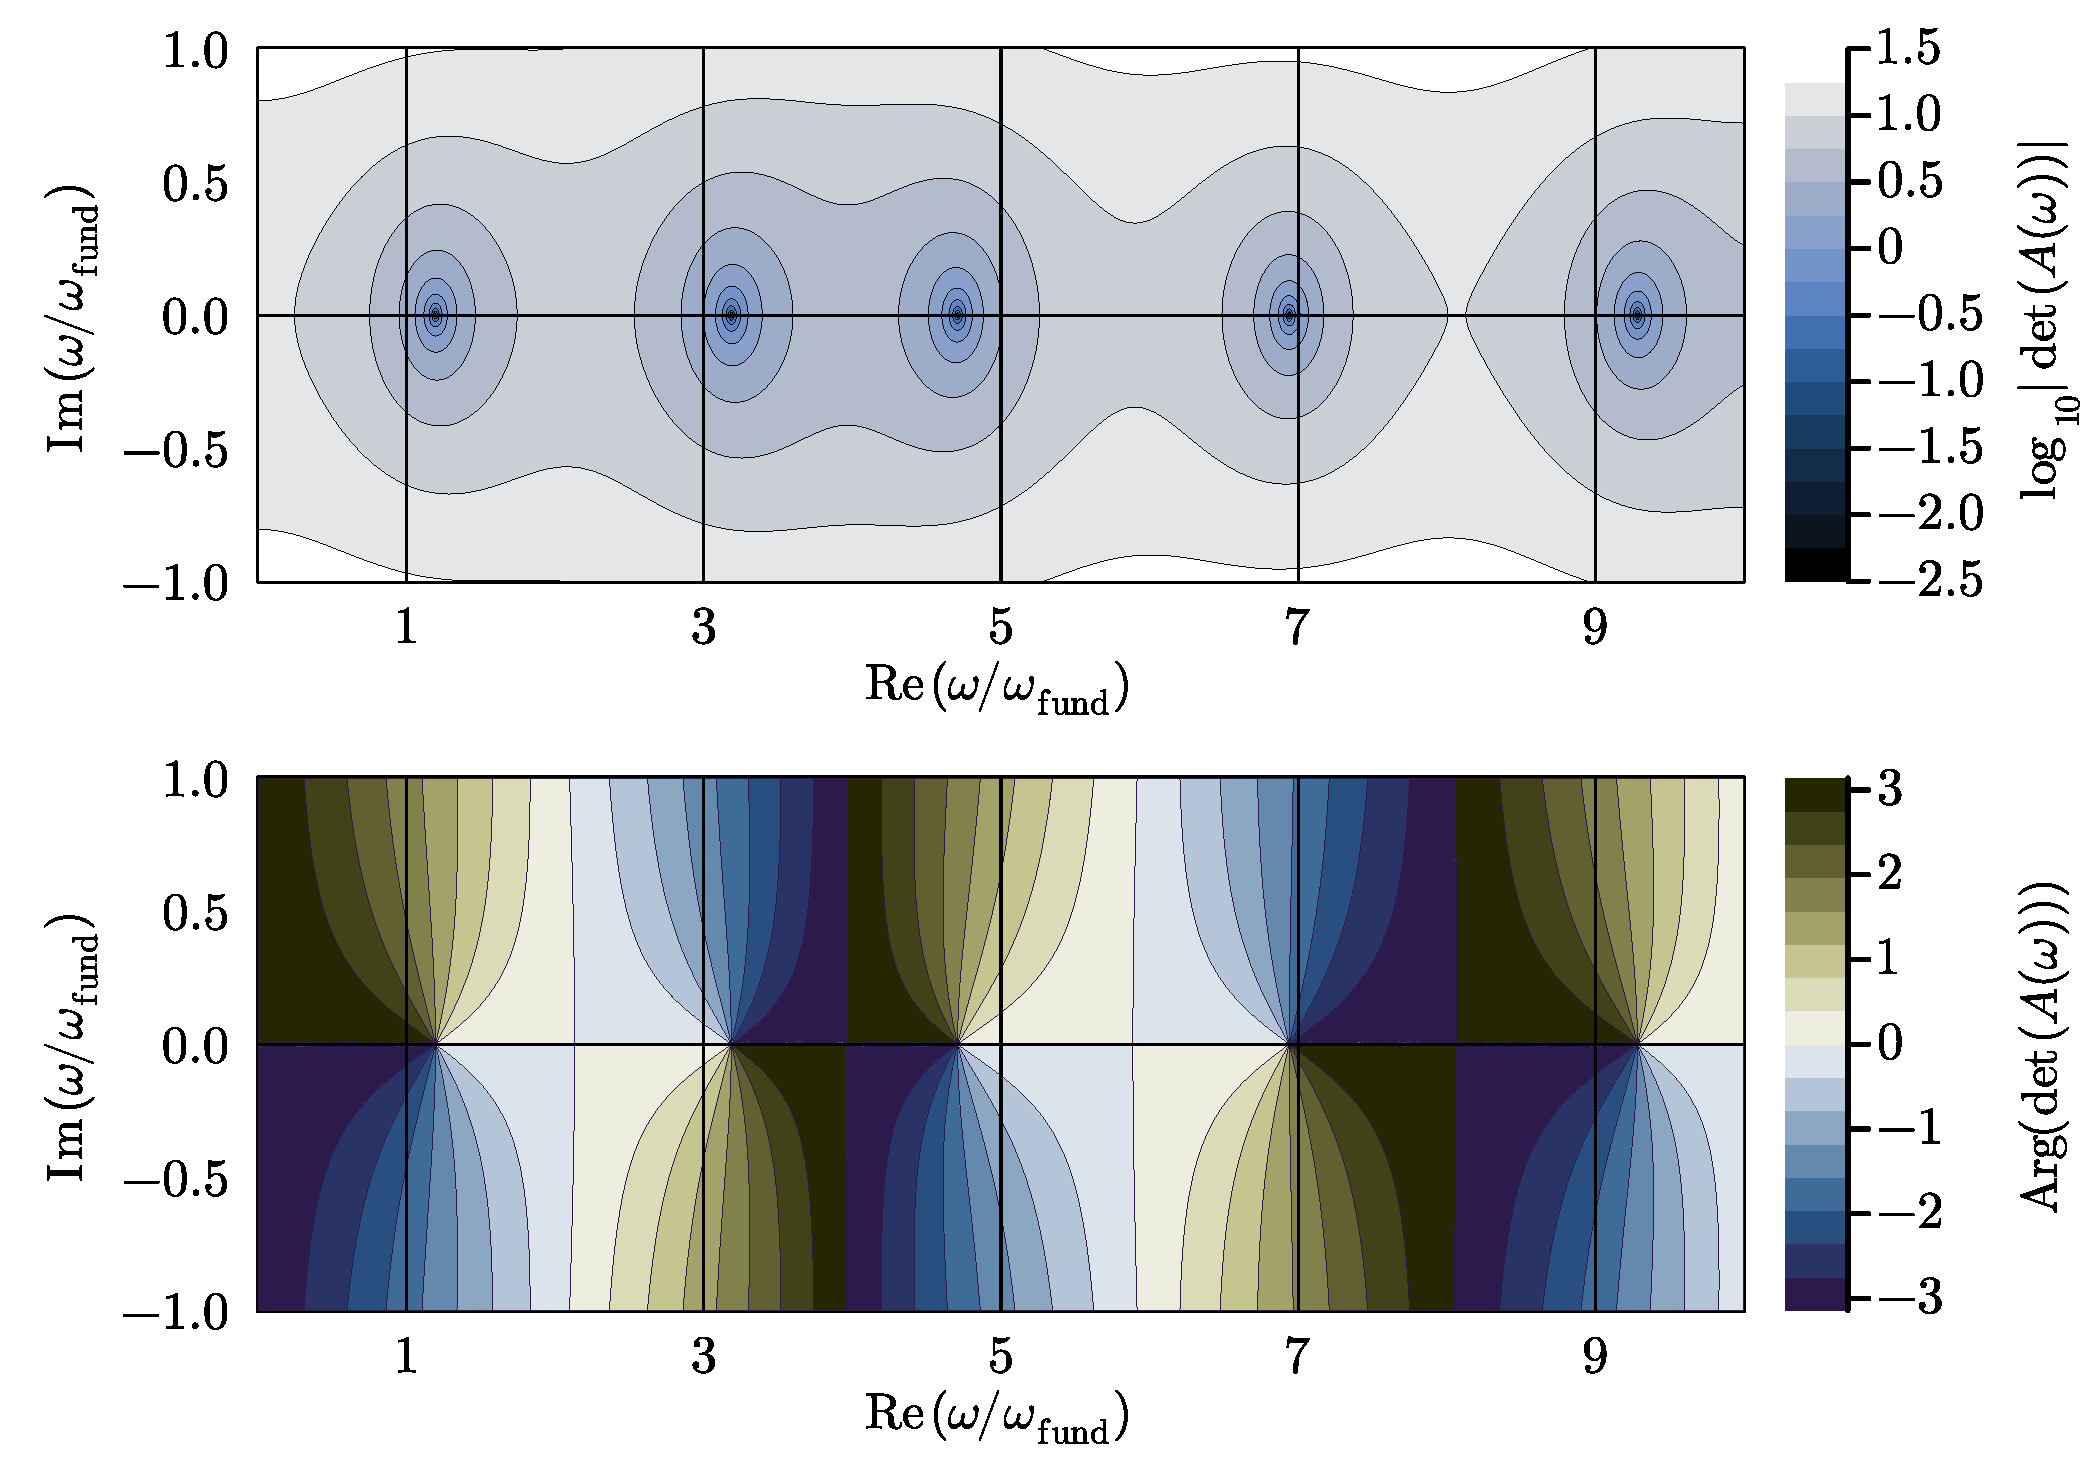
\includegraphics[scale=0.35]{assets/graphs/r=7_xf=05_complex_harmonics.pdf}
\caption{$r = 7, x_f = 0.5$, CAPTION}
\label{fig:flame-harmonics-complex}
\end{figure}

% For a flame which is .. and .., we expect harmonics of frequencies .. provided that the acoustics remain linear and are not interacting with the flame
% Note that this only accounts for the modes of a stationary density jump. If the flame is moving instead, the acoustic modes in the tube change with the moving flame. Hence the acoustics in the tube will be much more complex in this case in a way which is not predicted by this model. More complex control diagrams may be required to model the moving system instead.






% Show some fields at an example time for both simulations

% stats data fft postprocessing/windowing

% spectrogram results

% frequencies

% mode structures!



\begin{figure}[t]
\centering
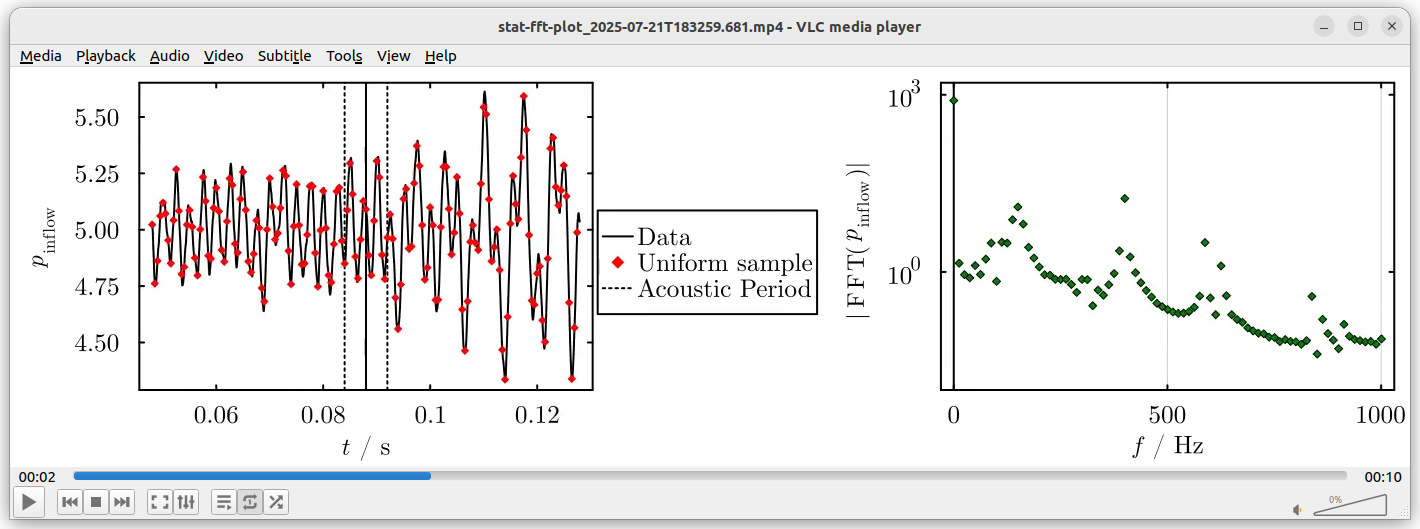
\includegraphics[scale=0.35]{assets/graphs/fft-windowing.png}
\caption{[PLACEHOLDER IMG] FFT WINDOWING}
\label{fig:windowing}
\end{figure}

\begin{figure}[t]
\centering
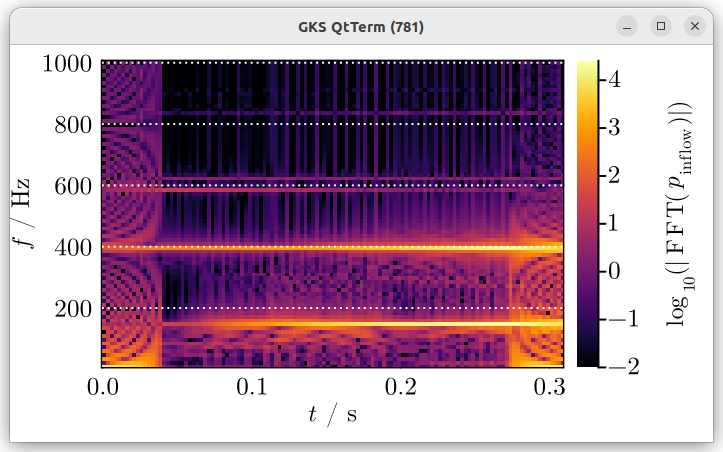
\includegraphics[scale=0.35]{assets/graphs/spectrogram.png}
\caption{[PLACEHOLDER IMG] SPECTROGRAM}
\label{fig:spectrogram}
\end{figure}

\begin{figure}[t]
\centering
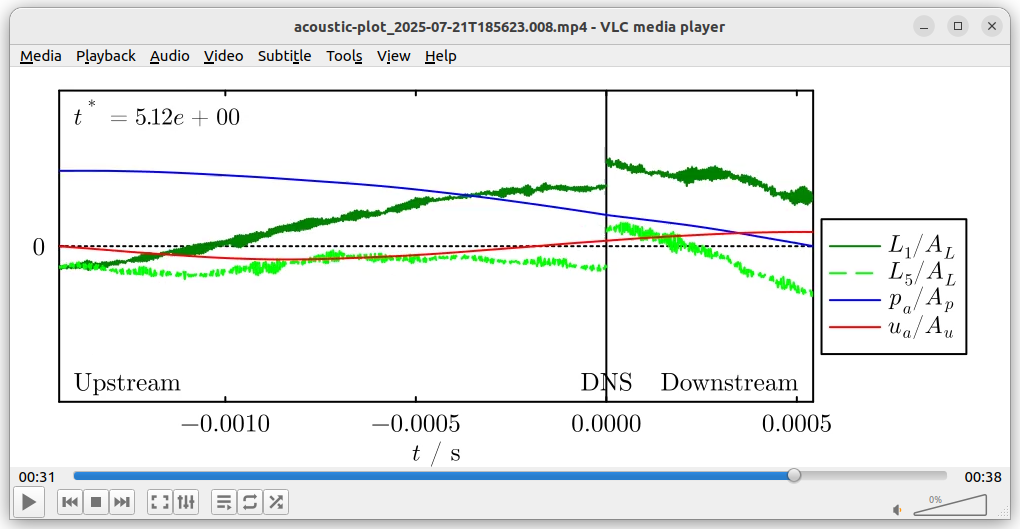
\includegraphics[scale=0.35]{assets/graphs/pp-tones.png}
\caption{[PLACEHOLDER IMG] POST-PROCESSED 1/4 AND 3/4 WAVE EVIDENCE}
\label{fig:pp-tones}
\end{figure}


